\chapter{Implementation of Ansieyes}

With the architecture defined, we moved to implementation. The entire system is written in Python and packaged for installation via pip. In this chapter, we describe the key algorithms and integration details. Due to confidentiality considerations, we present the logic in algorithmic form rather than as raw source code.

\section{Project Organisation}

Table \ref{tab:projstructure} lists the main directories and their roles.

\begin{table}[htb]
\centering
\renewcommand{\arraystretch}{1.3}
\setlength{\arrayrulewidth}{0.5mm}
\fontsize{10}{12}\selectfont
\caption[Project directory layout]{\textbf{Project directory layout}}
\vspace{2mm}
\label{tab:projstructure}
\begin{tabular}{|p{3.5cm}|p{8cm}|}
\hline
\textbf{Directory} & \textbf{Role} \\
\hline
\texttt{utils/} & Core library: analyser, models, security, duplicates \\
\hline
\texttt{cli/} & Command-line tools for all features \\
\hline
\texttt{tests/} & Unit and integration test suite \\
\hline
\texttt{cutlery/workflows/} & GitHub Actions workflow templates \\
\hline
\texttt{ui/} & Streamlit-based web interface (prototype) \\
\hline
\end{tabular}
\end{table}

After installation, four commands become available: \texttt{ai-triage} for issue analysis, \texttt{ai-triage-duplicate} for duplicate detection, \texttt{ai-triage-cosine} for offline similarity checking, and \texttt{ai-triage-pr} for pull request review.

\section{Core Analysis Engine}

The central class, \texttt{GeminiIssueAnalyser}, orchestrates the full analysis pipeline. Algorithm \ref{alg:analyse} outlines the process.

\begin{figure}[htb]
\centering
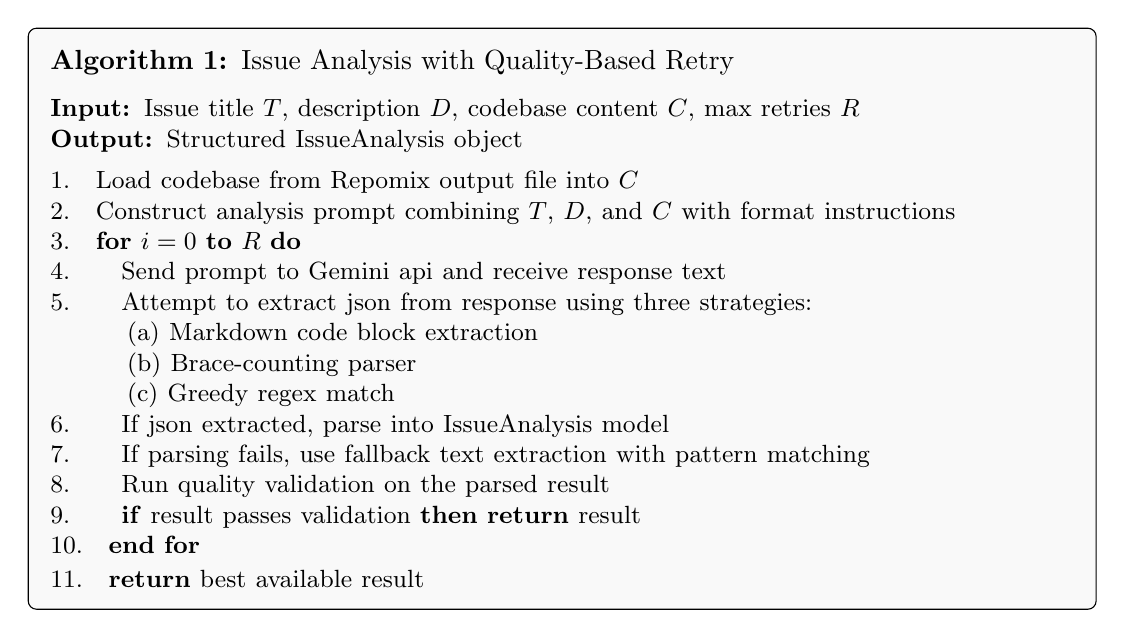
\begin{tikzpicture}
\node[draw, text width=13cm, inner sep=8pt, rounded corners=3pt, fill=gray!5] {
\textbf{Algorithm 1:} Issue Analysis with Quality-Based Retry\\[6pt]
\small
\textbf{Input:} Issue title $T$, description $D$, codebase content $C$, max retries $R$\\
\textbf{Output:} Structured IssueAnalysis object\\[4pt]
1.\quad Load codebase from Repomix output file into $C$\\
2.\quad Construct analysis prompt combining $T$, $D$, and $C$ with format instructions\\
3.\quad \textbf{for} $i = 0$ \textbf{to} $R$ \textbf{do}\\
4.\quad\quad Send prompt to Gemini \gls{api} and receive response text\\
5.\quad\quad Attempt to extract \gls{json} from response using three strategies:\\
\quad\quad\quad (a) Markdown code block extraction\\
\quad\quad\quad (b) Brace-counting parser\\
\quad\quad\quad (c) Greedy regex match\\
6.\quad\quad If \gls{json} extracted, parse into IssueAnalysis model\\
7.\quad\quad If parsing fails, use fallback text extraction with pattern matching\\
8.\quad\quad Run quality validation on the parsed result\\
9.\quad\quad \textbf{if} result passes validation \textbf{then return} result\\
10.\quad \textbf{end for}\\
11.\quad \textbf{return} best available result
};
\end{tikzpicture}
\label{alg:analyse}
\end{figure}

\subsection{Quality Validation}
We found early on that the model occasionally produces vague or incomplete analyses, especially for issues with sparse descriptions. To catch these, we run every response through a validation check before accepting it. An analysis is considered low quality if any of the following are true:

\begin{itemize}
\item It contains fewer than one proposed solution.
\item The confidence score is below 0.3.
\item File paths include placeholder text such as ``path/to/'' or ``example.py.''
\item The analysis summary is shorter than 20 characters.
\item The primary cause description is shorter than 10 characters.
\item Any solution description is shorter than 10 characters.
\end{itemize}

If a response fails this check, the system retries with the same prompt, up to a configurable limit (default: 2 retries). In our testing, most low-quality responses were corrected on the first retry.

\subsection{Prompt Design}
The analysis prompt is built from four parts: a system role statement (``You are an expert software engineer analysing a code issue''), the issue title and description, the full codebase content, and detailed instructions specifying the expected \gls{json} output format. We also include guidelines telling the model to use diff-style code changes, reference actual files from the codebase, and acknowledge when it is uncertain rather than guessing.

Custom prompts can be loaded from a file, allowing teams to tailor the analysis for their specific domain or conventions.

\section{Prompt Injection Detection}

The security module runs before any issue reaches the analyser. Algorithm \ref{alg:injection} describes the multi-layered detection process.

\begin{figure}[htb]
\centering
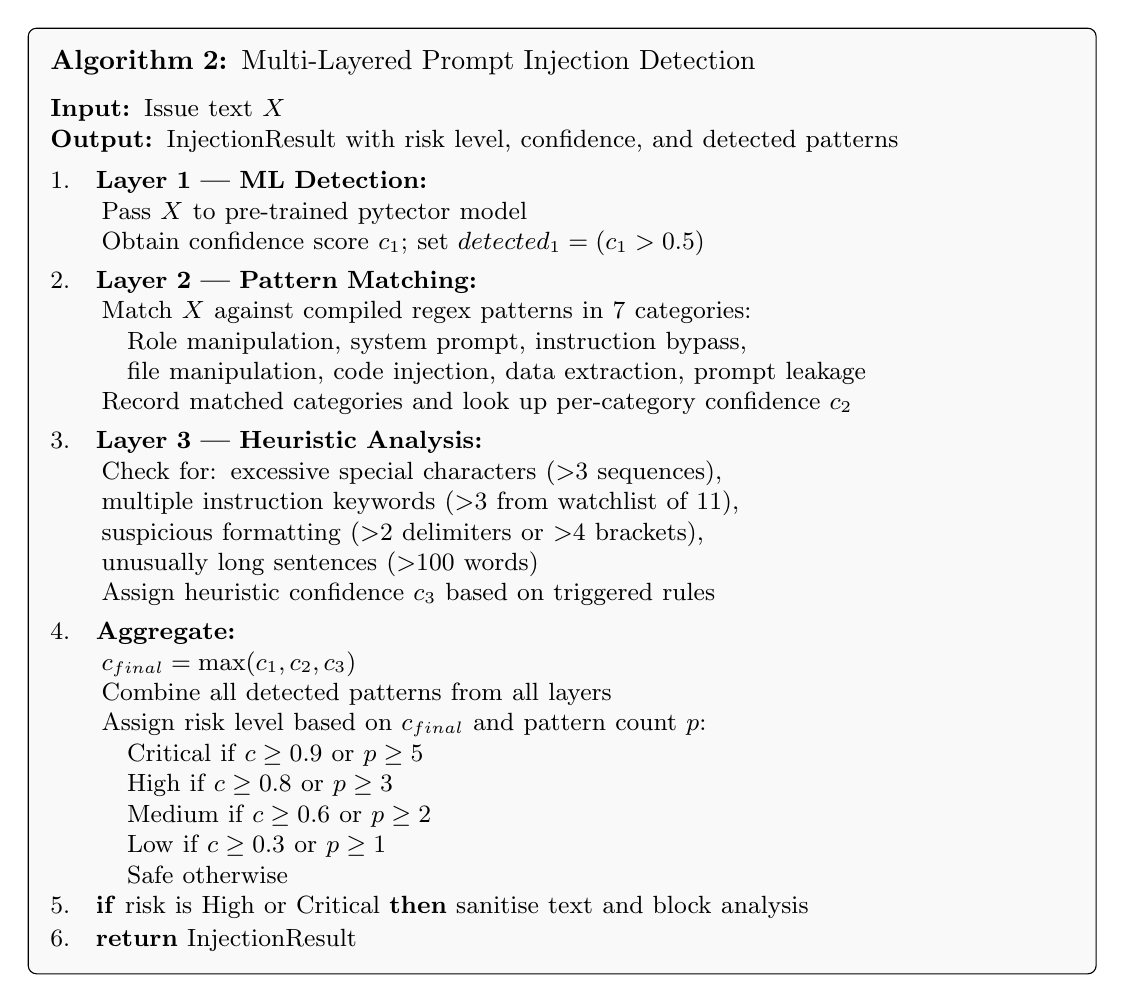
\begin{tikzpicture}
\node[draw, text width=13cm, inner sep=8pt, rounded corners=3pt, fill=gray!5] {
\textbf{Algorithm 2:} Multi-Layered Prompt Injection Detection\\[6pt]
\small
\textbf{Input:} Issue text $X$\\
\textbf{Output:} InjectionResult with risk level, confidence, and detected patterns\\[4pt]
1.\quad \textbf{Layer 1 --- ML Detection:}\\
\quad\quad Pass $X$ to pre-trained pytector model\\
\quad\quad Obtain confidence score $c_1$; set $\text{detected}_1 = (c_1 > 0.5)$\\[3pt]
2.\quad \textbf{Layer 2 --- Pattern Matching:}\\
\quad\quad Match $X$ against compiled regex patterns in 7 categories:\\
\quad\quad\quad Role manipulation, system prompt, instruction bypass,\\
\quad\quad\quad file manipulation, code injection, data extraction, prompt leakage\\
\quad\quad Record matched categories and look up per-category confidence $c_2$\\[3pt]
3.\quad \textbf{Layer 3 --- Heuristic Analysis:}\\
\quad\quad Check for: excessive special characters ($>$3 sequences),\\
\quad\quad multiple instruction keywords ($>$3 from watchlist of 11),\\
\quad\quad suspicious formatting ($>$2 delimiters or $>$4 brackets),\\
\quad\quad unusually long sentences ($>$100 words)\\
\quad\quad Assign heuristic confidence $c_3$ based on triggered rules\\[3pt]
4.\quad \textbf{Aggregate:}\\
\quad\quad $c_{\text{final}} = \max(c_1, c_2, c_3)$\\
\quad\quad Combine all detected patterns from all layers\\
\quad\quad Assign risk level based on $c_{\text{final}}$ and pattern count $p$:\\
\quad\quad\quad Critical if $c \geq 0.9$ or $p \geq 5$\\
\quad\quad\quad High if $c \geq 0.8$ or $p \geq 3$\\
\quad\quad\quad Medium if $c \geq 0.6$ or $p \geq 2$\\
\quad\quad\quad Low if $c \geq 0.3$ or $p \geq 1$\\
\quad\quad\quad Safe otherwise\\
5.\quad \textbf{if} risk is High or Critical \textbf{then} sanitise text and block analysis\\
6.\quad \textbf{return} InjectionResult
};
\end{tikzpicture}
\label{alg:injection}
\end{figure}

The pattern matching layer deserves some additional detail. Table \ref{tab:patterns} lists the seven categories and representative patterns.

\begin{table}[htb]
\centering
\renewcommand{\arraystretch}{1.3}
\setlength{\arrayrulewidth}{0.5mm}
\fontsize{10}{12}\selectfont
\caption[Prompt injection pattern categories and assigned confidence levels]{\textbf{Prompt injection pattern categories and assigned confidence levels}}
\vspace{2mm}
\label{tab:patterns}
\begin{tabular}{|p{3cm}|p{5.5cm}|c|}
\hline
\textbf{Category} & \textbf{Example Patterns} & \textbf{Confidence} \\
\hline
Instruction bypass & ``bypass security,'' ``jailbreak'' & 0.95 \\
\hline
Role manipulation & ``ignore previous instructions,'' ``you are now'' & 0.90 \\
\hline
Prompt leakage & ``show original prompt,'' ``reveal system prompt'' & 0.90 \\
\hline
Code injection & ``eval(,'' ``exec(,'' \texttt{<script>} & 0.85 \\
\hline
System prompts & ``system:,'' ``[system],'' \texttt{```system} & 0.80 \\
\hline
Data extraction & ``show password,'' ``reveal token'' & 0.80 \\
\hline
File manipulation & ``create file,'' ``write to file'' & 0.75 \\
\hline
\end{tabular}
\end{table}

The heuristic layer watches for 11 specific keywords: \textit{ignore, forget, disregard, override, bypass, system, assistant, admin, root, jailbreak, unrestricted}. Seeing three or more of these in a single issue raises the heuristic confidence to 0.7.

\section{Duplicate Detection}

\subsection{Gemini-Based Detection}
Algorithm \ref{alg:geminidup} describes the semantic approach.

\begin{figure}[htb]
\centering
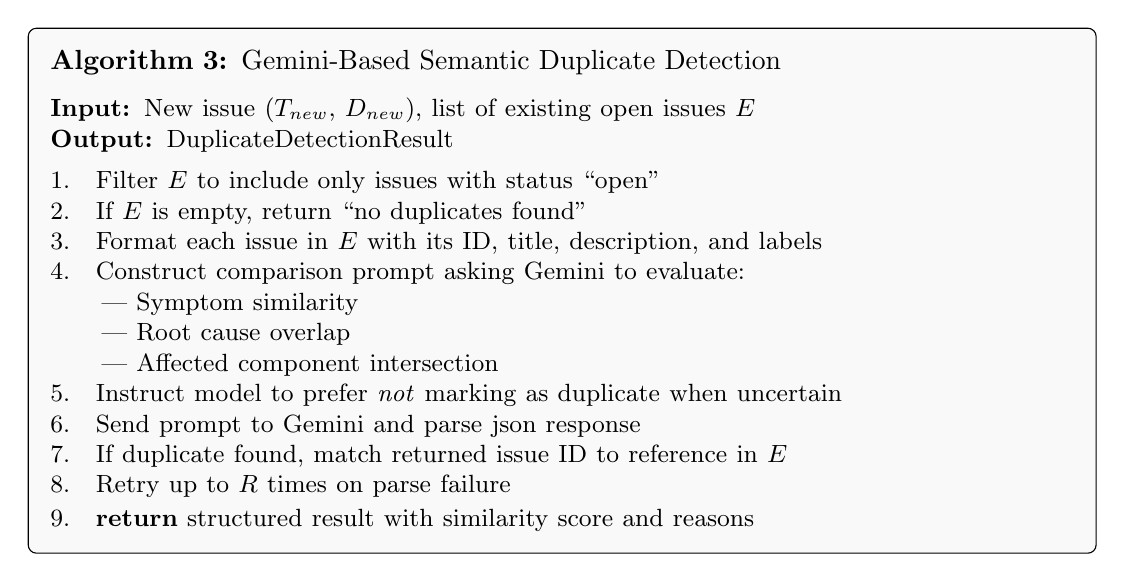
\begin{tikzpicture}
\node[draw, text width=13cm, inner sep=8pt, rounded corners=3pt, fill=gray!5] {
\textbf{Algorithm 3:} Gemini-Based Semantic Duplicate Detection\\[6pt]
\small
\textbf{Input:} New issue ($T_{\text{new}}$, $D_{\text{new}}$), list of existing open issues $E$\\
\textbf{Output:} DuplicateDetectionResult\\[4pt]
1.\quad Filter $E$ to include only issues with status ``open''\\
2.\quad If $E$ is empty, return ``no duplicates found''\\
3.\quad Format each issue in $E$ with its ID, title, description, and labels\\
4.\quad Construct comparison prompt asking Gemini to evaluate:\\
\quad\quad --- Symptom similarity\\
\quad\quad --- Root cause overlap\\
\quad\quad --- Affected component intersection\\
5.\quad Instruct model to prefer \textit{not} marking as duplicate when uncertain\\
6.\quad Send prompt to Gemini and parse \gls{json} response\\
7.\quad If duplicate found, match returned issue ID to reference in $E$\\
8.\quad Retry up to $R$ times on parse failure\\
9.\quad \textbf{return} structured result with similarity score and reasons
};
\end{tikzpicture}
\label{alg:geminidup}
\end{figure}

\subsection{Cosine Similarity Detection}
Algorithm \ref{alg:cosinedup} describes the offline approach.

\begin{figure}[htb]
\centering
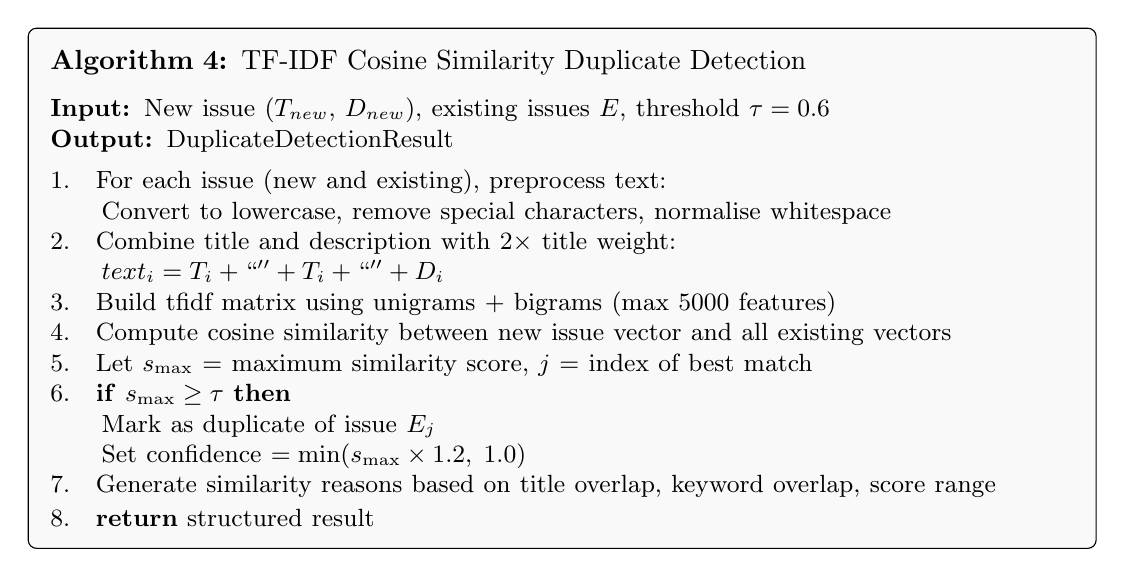
\begin{tikzpicture}
\node[draw, text width=13cm, inner sep=8pt, rounded corners=3pt, fill=gray!5] {
\textbf{Algorithm 4:} TF-IDF Cosine Similarity Duplicate Detection\\[6pt]
\small
\textbf{Input:} New issue ($T_{\text{new}}$, $D_{\text{new}}$), existing issues $E$, threshold $\tau = 0.6$\\
\textbf{Output:} DuplicateDetectionResult\\[4pt]
1.\quad For each issue (new and existing), preprocess text:\\
\quad\quad Convert to lowercase, remove special characters, normalise whitespace\\
2.\quad Combine title and description with 2$\times$ title weight:\\
\quad\quad $\text{text}_i = T_i + \text{`` ''} + T_i + \text{`` ''} + D_i$\\
3.\quad Build \gls{tfidf} matrix using unigrams + bigrams (max 5000 features)\\
4.\quad Compute cosine similarity between new issue vector and all existing vectors\\
5.\quad Let $s_{\max}$ = maximum similarity score, $j$ = index of best match\\
6.\quad \textbf{if} $s_{\max} \geq \tau$ \textbf{then}\\
\quad\quad Mark as duplicate of issue $E_j$\\
\quad\quad Set confidence $= \min(s_{\max} \times 1.2,\; 1.0)$\\
7.\quad Generate similarity reasons based on title overlap, keyword overlap, score range\\
8.\quad \textbf{return} structured result
};
\end{tikzpicture}
\label{alg:cosinedup}
\end{figure}

\section{Librarian--Surgeon Implementation}

The Librarian processes the codebase in chunks. For each directory-level chunk, it sends a targeted prompt to Gemini asking which files are relevant to the issue. Responses are validated by checking that each returned path contains a directory separator, has a file extension, does not start with a comment marker, and is no longer than 200 characters. Paths that fail these checks are discarded.

Once the Librarian produces its final file list, a targeted Repomix output is generated containing only those files. The Surgeon then runs the standard analysis pipeline (Algorithm 1) against this focused context.

\section{GitHub Actions Integration}

The single-issue workflow follows this sequence:

\begin{enumerate}
\item Check out the repository and set up the Python environment.
\item Generate a Repomix output from the remote repository URL.
\item Run the prompt injection detector on the issue content.
\item If the risk is High or Critical, post a security alert comment and stop.
\item Fetch all existing open issues (older than the current one).
\item Run duplicate detection against the existing issues.
\item If a duplicate is found, post a comment linking to the original and stop.
\item Run the full Gemini analysis.
\item Parse the analysis output and post it as a formatted comment on the issue.
\item Apply labels for issue type (e.g., ``type:bug'') and severity (e.g., ``severity:high'').
\item Upload analysis artefacts (results, logs, configuration) with 30-day retention.
\end{enumerate}

The bulk analysis workflow follows a similar pattern but iterates over all open issues, processing them from oldest to newest. This ordering matters for duplicate detection: when we analyse issue \#5 before \#10, and \#10 turns out to be a duplicate, we can correctly point it to \#5 as the original.

\section{Configuration}

The system reads its settings from a \gls{json} file (\texttt{triage.config.json}) that specifies the repository URL, the path to the Repomix output, an optional custom prompt file, and the Gemini model to use. For \gls{pr} review, a separate \gls{yaml} file maps repository URL patterns to domain-specific review prompts---for instance, Python-focused repositories get prompts that emphasise PEP 8 compliance and docstring coverage.

\section{Testing}

We wrote tests across five modules covering data models, the core analyser, both duplicate detectors, and the \gls{pr} reviewer. Tests are tagged as \texttt{unit} (no \gls{api} key needed) or \texttt{integration} (requires a live Gemini key). The \gls{ci} pipeline runs unit tests across Python 3.11, 3.12, and 3.13 in parallel, alongside formatting checks (Black), import ordering (isort), and linting (Flake8). A single ``All Checks Pass'' gate prevents merging code that fails any of these.

The algorithms and integration points described here realise the architecture from the previous chapter. We now turn to how well the system performs in practice.

\section{Summary}

This chapter detailed the implementation of Ansieyes, presenting the key algorithms for issue analysis with quality-based retry, multi-layered prompt injection detection, both Gemini-based and cosine similarity duplicate detection, the Librarian--Surgeon two-pass pipeline, GitHub Actions integration, configuration management, and the testing infrastructure. The next chapter covers the testing and validation procedures used to verify the system's correctness and reliability.
